\documentclass{article}
\usepackage[english,russian]{babel}
\usepackage[utf8]{inputenc}
\usepackage{indentfirst}
\usepackage{graphicx}
\usepackage{float}
\usepackage[margin=2cm]{geometry}

\begin{document}
    \begin{titlepage}
        \begin{center}
            ГУАП
            \vspace{0.25cm}

            КАФЕДРА №51
        \end{center}

        \begin{flushleft}

            КУРСОВАЯ РАБОТА (ПРОЕКТ)

            ЗАЩИЩЕН С ОЦЕНКОЙ

            ПРЕПОДАВАТЕЛЬ


            \vspace{0.5cm}

            $\rule{5cm}{0.15mm}$ \hfill $\rule{2.2cm}{0.15mm}$  \hfill $\rule{3.25cm}{0.15mm}$

            должность, уч. степень, звание \hfill подпись, дата \hfill инициалы, фамилия
        \end{flushleft}

		\vspace{2cm}

        \begin{center}
            ПОЯСНИТЕЛЬНАЯ ЗАПИСКА\\
			К КУРСОВОЙ РАБОТЕ (ПРОЕКТУ)


            \vspace{1cm}
			
			Почтовый сервис ZenMail

            \vspace{1cm}

            по курсу: ОСНОВЫ ПРОГРАММИРОВАНИЯ {\MakeUppercase{\romannumeral 2}}
        \end{center}

        \vspace{6cm}

        \begin{flushleft}
            РАБОТУ ВЫПОЛНИЛ

            СТУДЕНТ ГР. № 5511 \hfill $\rule{2.2cm}{0.15mm}$  \hfill $\rule{3.25cm}{0.15mm}$

            \hspace{7.8cm} подпись, дата \hfill инициалы, фамилия
        \end{flushleft}

        \vspace{5cm}
        \begin{center}
            Санкт-Петербург 2017
        \end{center}
    \end{titlepage}
    
\newpage
\tableofcontents
\newpage

\section{Функциональная спецификация}
\subsection{Цель}
В качестве основной цели данной курсовой работы была поставлена разработка почтового сервиса с выделенной базой данных, почтовым сервером и функционально полным веб-приложением, позволяющим принимать и отправлять письма зарегестрированным пользователям. \\

Следовательно в данном случае необходимо было заняться многими направлениями разработки, и разбить большой объем работ над веб-приложением. Так сформировалась команда из трех человек: Андрей Щипило, Артем Заболотный и Сергей Костин. \\

Тогда весь объем работы разбивается на три главных компонента: 
\begin{itemize}
	\item \textbf{Интерактивная часть веб-приложения} –- интерактивная оболочка, созданная при помощи фреймворка Angular 2+. (далее frontend)

	\item \textbf{Программно-аппаратная часть веб-приложения} –- программа на фреймворке Spring с архитектурой REST, управляющая данными с frontend. (далее backend)

	\item \textbf{Почтовый сервер с базой данных} –- сервер, отвечающий за отправку, прием и хранение писем. (далее mailserver)
\end{itemize}


\textbf{Frontend}: это интерфейс взаимодейтсвия между пользователем и программно-аппаратной частью веб-приложения, использующий веб-технологии для обработки информации полученной от пользователя на клиенете или отправляя информацию на \emph{Backend}, предоставляя пользователю полный контроль над своим почтовым ящиком, включая регистрации, аутентификацию, а также просмотр и отправку сообщений. \\

\textbf{Backend}: это программа, исполняющаяся на пердполагаемом сервере, которая обрабатывает информацию и отвечает на запросы от \emph{Frontend}, выполняя необходимые действия (прим. добавление нового пользователя в базу данных). Для улучшения опыта использования веб-приложения сервер должен своевременно и быстро обрабатывать запросы от нескольких пользователей одновременно. Именно с этого приложения происходит запросы почтовому серверу на отправку и чтение писем, по протоколам IMAP, POP3 и SMTP. \\

\textbf{Mail Server}: это специально настроенный сервер, размещенный на сервере, который может быть использован большую часть времени (прим. облачное хранилище). На машине в облаке установлены и конфигурированы программы для отправки и принятия писем, проверки писем на спам, вирусы, а также для аутентификации и шифрования соединений. Причем именно на этом сервер хранится и база данных, с которой активно взаимодействует \emph{Frontend} часть веб-приложения. \\

\subsection{Основные функции}

Основные функции программы:

\begin{itemize}
  \item Возможность подключения к почтовому серверу не только с реализованного в курсовой работе веб-приложения
  \item Регистрация новых пользователей через форму.
  \item Вход в почтовый ящик по логину и паролю.
  \item Просмотр пришедших писем.
  \item Поиск по письмам.
  \item Создание нового письма с базовым редактированием.
\end{itemize}

\subsection{Технологии}

\begin{table}[]
\centering
\begin{tabular}{|l|l|}
\hline
\multicolumn{1}{|c|}{\textbf{Component}} & \multicolumn{1}{c|}{\textbf{Technology}} \\ \hline
Frontend                                 & Angular 4+ and Covalent                  \\
Backend (REST)                           & SpringBoot (Java)                        \\
Security                                 & Token                                    \\
In Memory DB                             & H2                                       \\
Persistence                              & JPA (Using Spring Data)                  \\
Client Build Tools                       & angular-cli, Webpack, npm                \\
Server Build Tools                       & Maven (Java)                             \\ \hline
\end{tabular}
\caption{Стэк технологий}
\label{my-label}
\end{table}

Кроме основного стэка технологий будут использоваться дополнительные сторонние разработки и программы для обеспечения быстроты, удобства разработки и использования, а также общей безопасности системы: \\

\begin{itemize}
\item Ubuntu Server 16.04 LTS
\item Postfix, MTA
\item Dovecot
\item MySQL
\item Rspamd
\item Amazon EC2
\end{itemize}

\subsection{Команда}
Так как существовали установленные сроки сдачи курсовой работы, необходимо было распределить курс работ равномерно между всеми участниками проекта, чтобы максимизировать участие каждого из участников в проекте и минимизировать время затраченное в ожидании результатов одного из участников.
В конечном итоге было предложено такое распределение по обязанностям:
\begin{itemize}
\item Щипило Андрей: занимается общей архитектурой веб-приложения SpringFramework, правильной инициализацией процессов приложения через SpringBoot и Maven, графическим и пользовательским представлением веб-приложения, используя возможности Angular 4, менеджментом проекта, а также настройкой и поддержанием почтового сервера в облачном хранилище.

\item Костин Сергей: занимается обработкой данных почтового сервера и веб-приложения, используя MariaDB и Spring Data, представлением данных в программе, а отвечает за безопасную аутентификацию пользователей через токены и фильтры безопасности системы, используя Spring Security и защищеные протоколы связи.

\item Заболотный Артем: занимается связью между программной и графической частями приложения, используя нативный для Angular 4 язык программированния TypeScript,  из Spring Security, является менеджером глобального тестирования веб-приложения, а также за защищенную связь через почтовые протоколы IMAPS и SMTPS, позволяющую безопасно связать программную часть веб-приложения и почтовый сервер.
\end{itemize}
\newpage

\section{Руководство пользователя}

\subsection{Авторизация}
После перехода на адрес веб-приложения пользователя перенаправят на страницу авторизации.
\begin{figure}[H]
        \begin{flushleft}
            \centerline{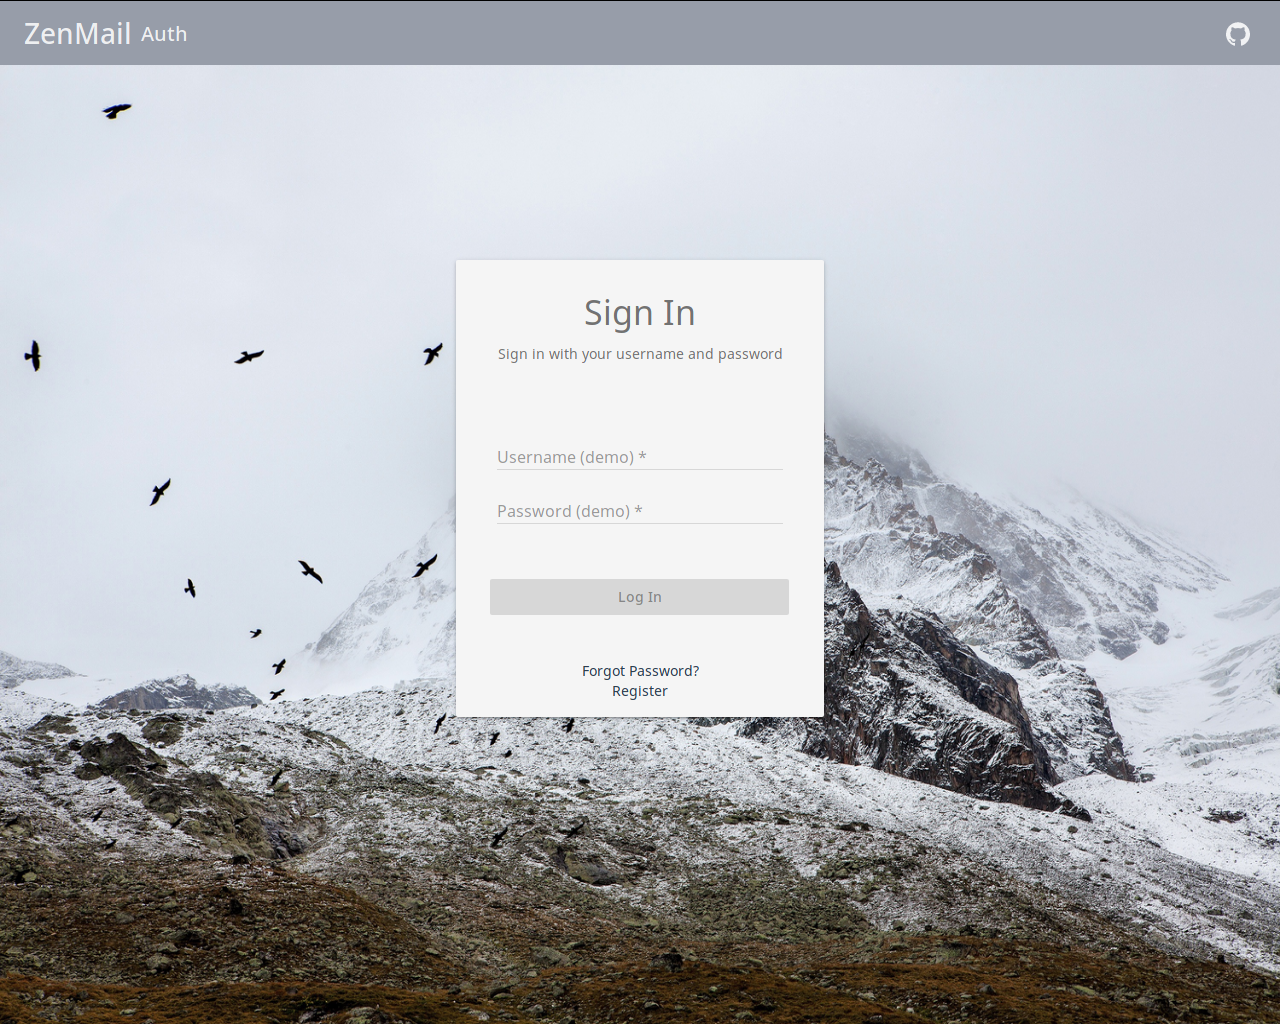
\includegraphics[scale=0.6]{loginscreen.png}}
            \caption{Страница авторизации}
        \end{flushleft}
\end{figure}

Если у пользователя нет действующей почты он может перейти на страницу регистрации, нажав на ссылку Register.

\begin{figure}[H]
        \begin{flushleft}
            \centerline{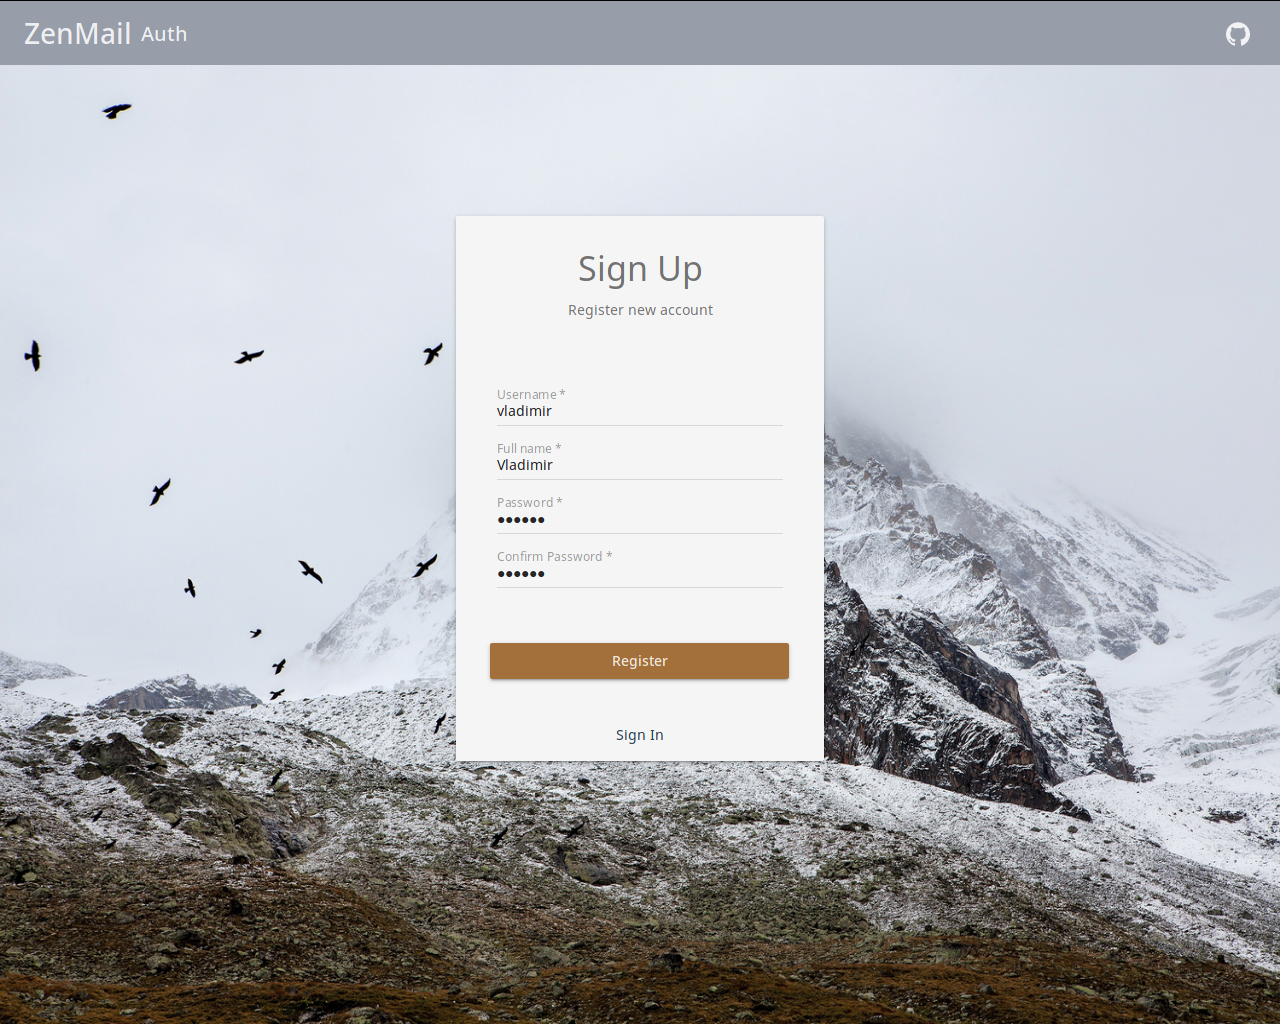
\includegraphics[scale=0.6]{register.png}}
            \caption{Страница регистрации}
        \end{flushleft}
\end{figure}

После верного заполнения всех полей пользователя перенаправит на главную страницу с письмами.
\begin{figure}[H]
        \begin{flushleft}
            \centerline{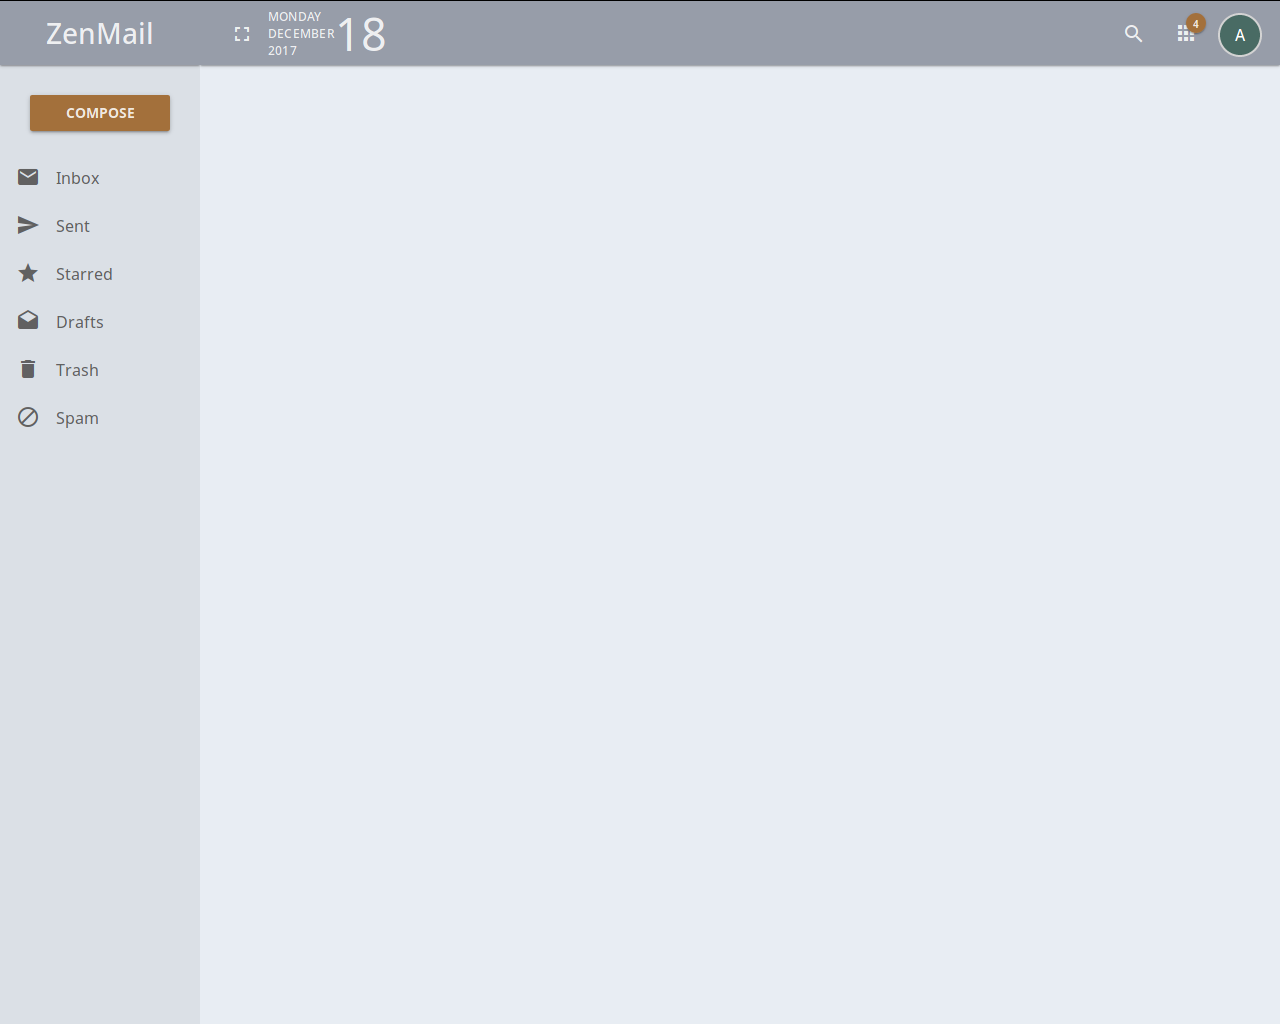
\includegraphics[scale=0.6]{homescreen.png}}
            \caption{Домашняя страница авторизированного аккаунта}
        \end{flushleft}
\end{figure}

После перехода на домашнюю страницу пользователь может управлять своим почтовым аккаунтом. \\

\subsection{Входящие сообщения}
При нажатии на кнопку Inbox открывается страница со всеми входящими сообщениями на данном аккаунте.

\begin{figure}[H]
        \begin{flushleft}
            \centerline{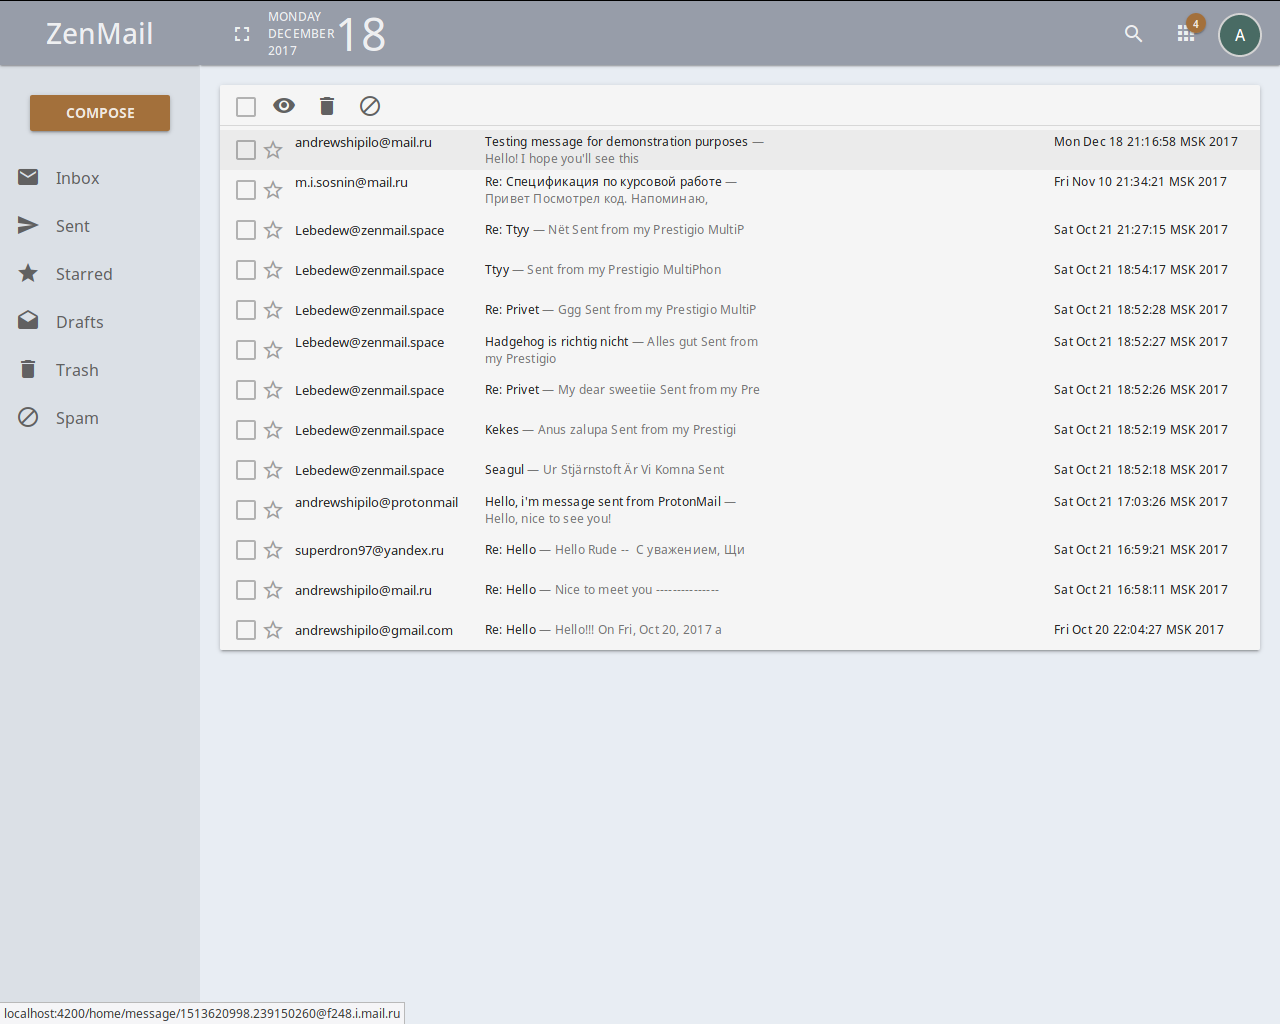
\includegraphics[scale=0.6]{inbox.png}}
            \caption{Входящие сообщения}
        \end{flushleft}
\end{figure}

При нажатии на любое из сообщений мы можем открыть его 

\begin{figure}[H]
        \begin{flushleft}
            \centerline{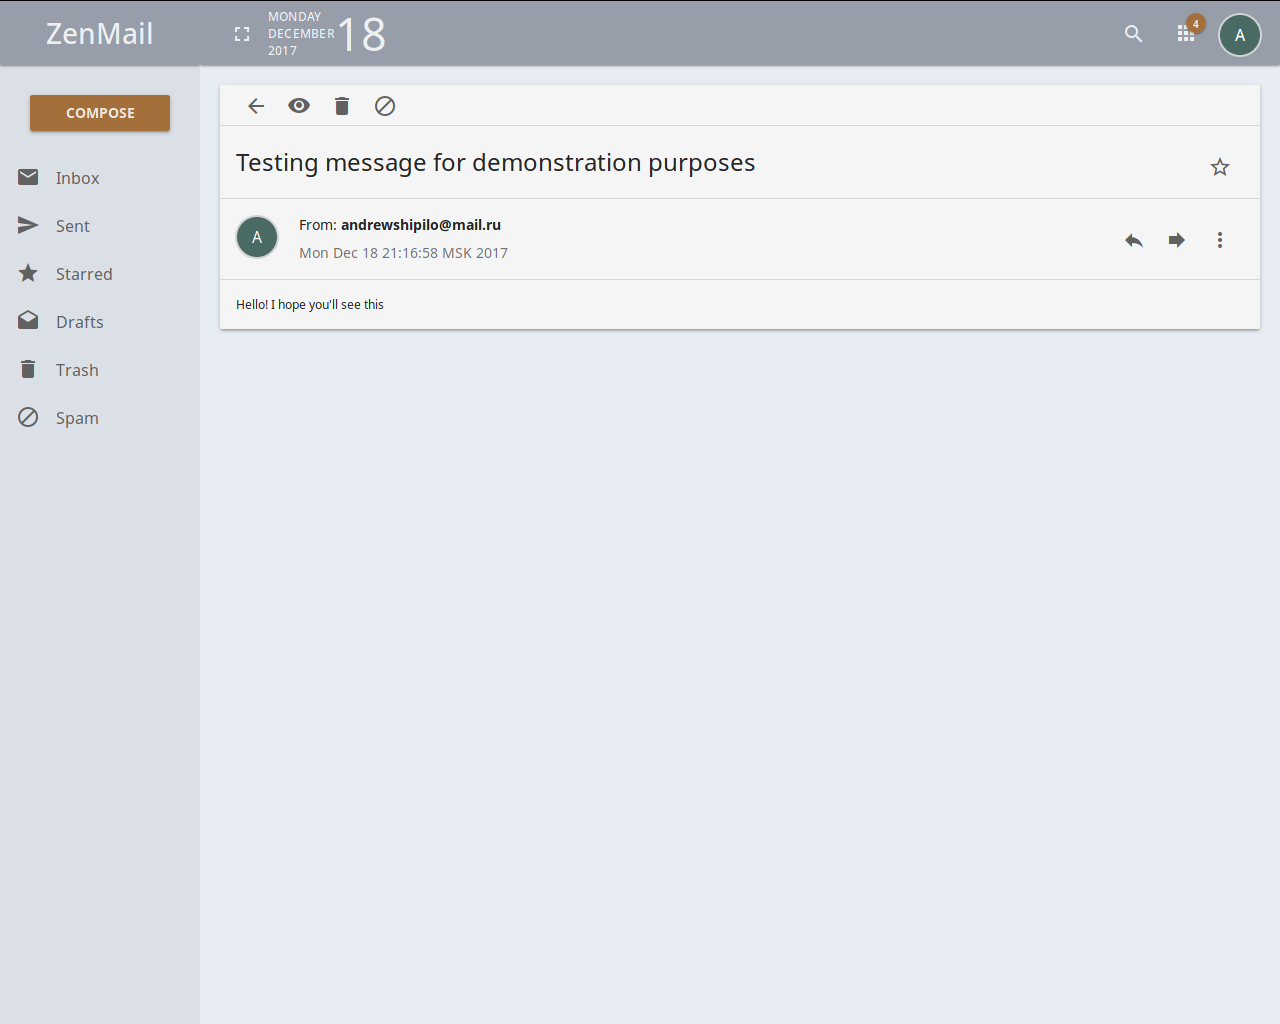
\includegraphics[scale=0.6]{message.png}}
        \caption{Содержимое сообщения}
        \end{flushleft}
\end{figure}

\subsection{Отправка сообщения}
Для того, чтобы отправить сообщение нужно нажать на кнопку COMPOSE, после этого появится форма отправки сообщения, где можно указать получателя, тему и текст сообщения. Эту форму можно закрыть, нажав на крестик в правом углу. Для того, чтобы отправить сообщение необходимо нажать на самолетик.

\begin{figure}[H]
        \begin{flushleft}        \centerline{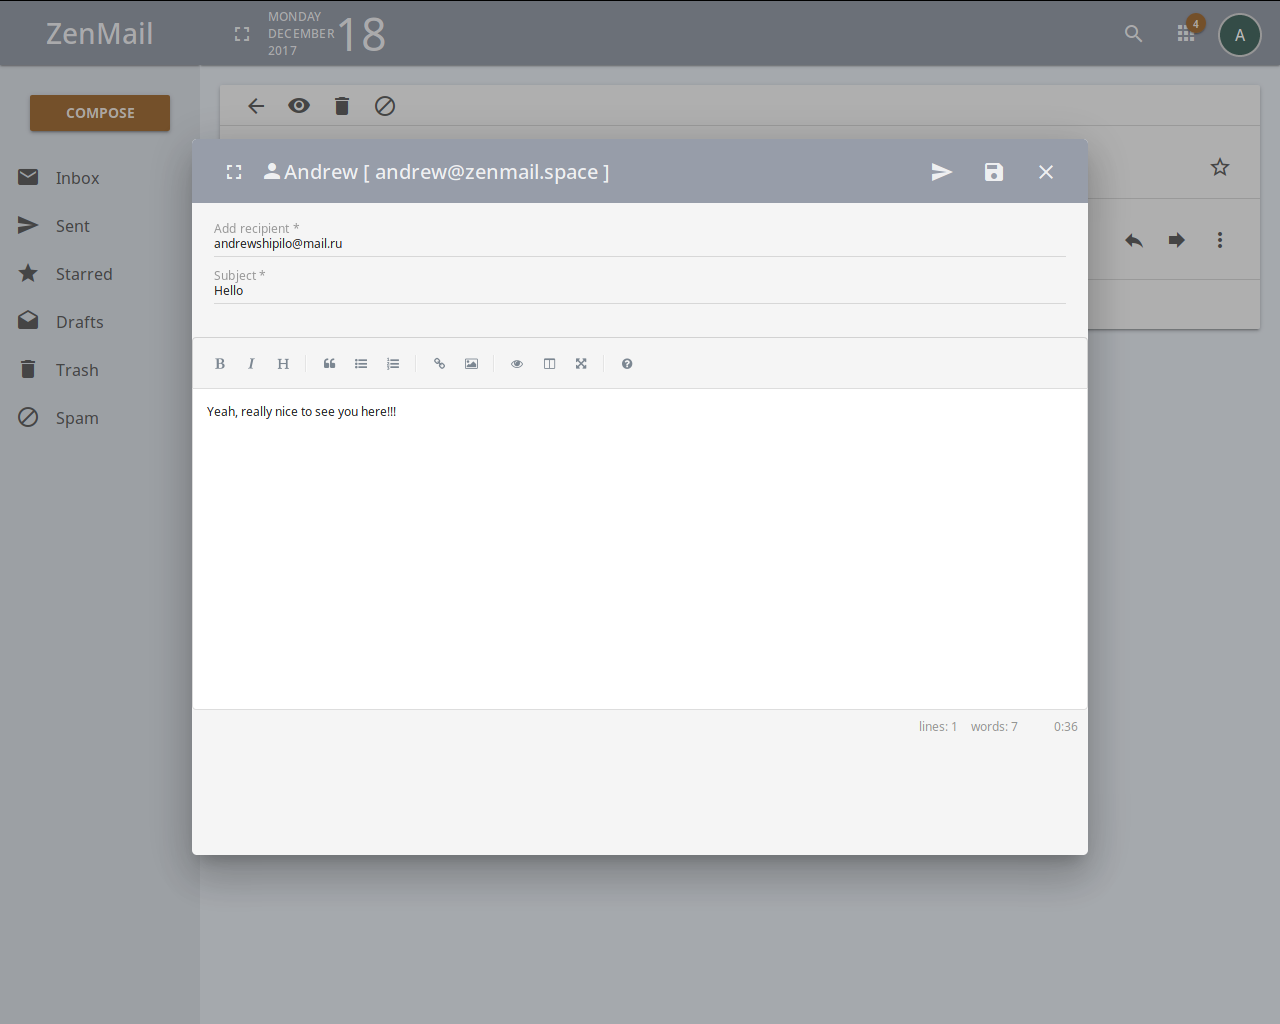
\includegraphics[scale=0.6]{sendmessage.png}}
        \caption{Форма отправки сообщения}
        \end{flushleft}
\end{figure}

При отправке сообщения форма закроется и появится уведомление с результатом отправки сообщения.

\begin{figure}[H]
        \begin{flushleft}        \centerline{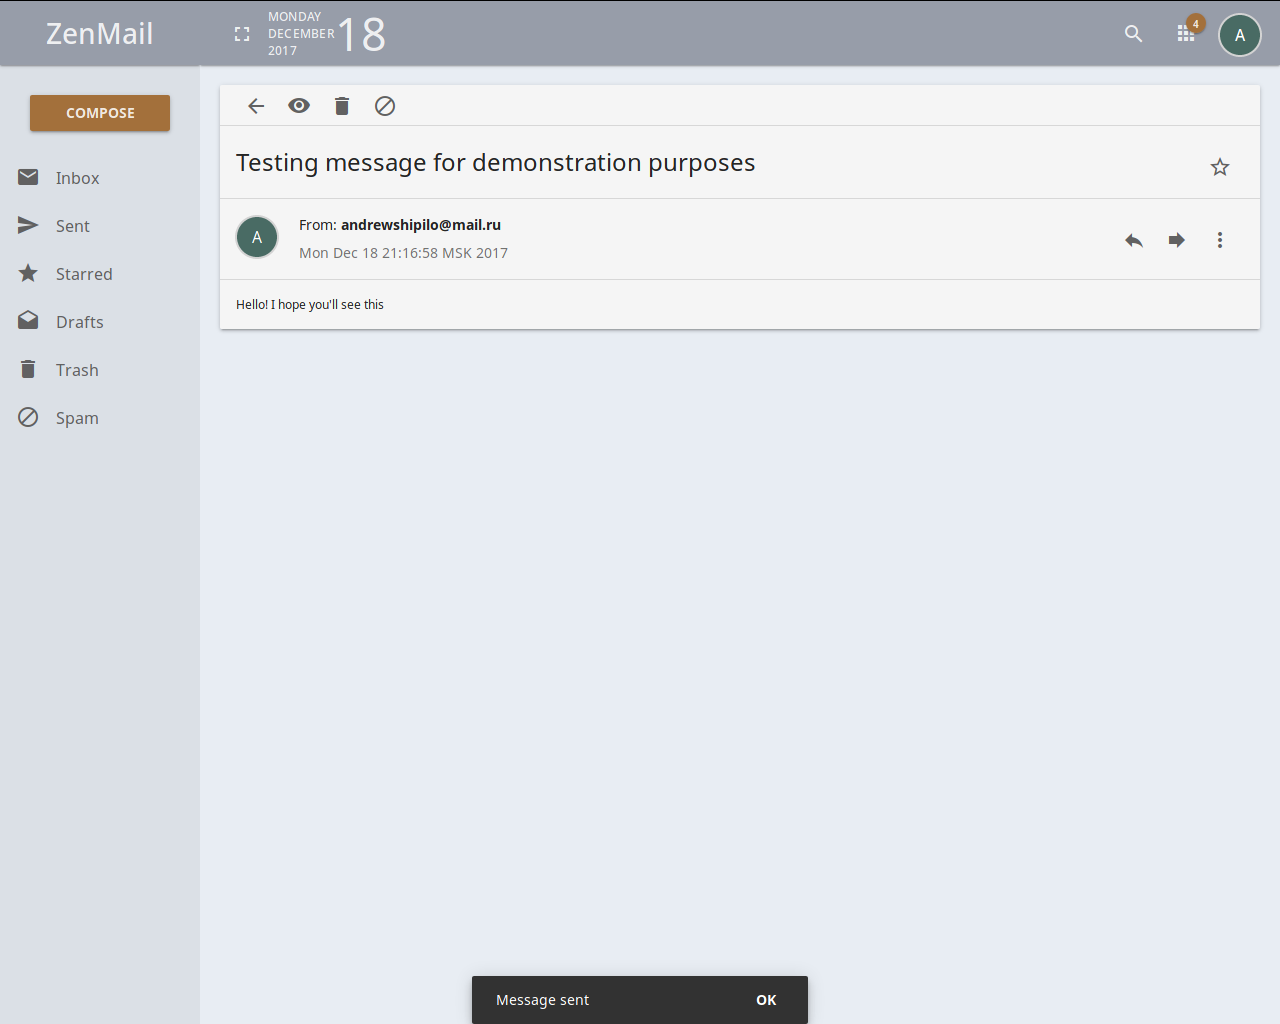
\includegraphics[scale=0.6]{messagesent.png}}
        \caption{Уведомление об отправке сообщения}
        \end{flushleft}
\end{figure}

\newpage

\section{Описание архитектуры проекта}
Проект, как говорилось раньше, можно разделить на три главные составляющие: Frontend, Backend и MailServer. В общем виде Frontend посылает запрос Backend'у, и в большинстве случаев Backend посылает запрос базе, получает ответ, обрабатывает и отсылает на Frontend. \\
Общее взаимодействие между основными компонентами проекта можно наблюдать на схеме ниже. 

\begin{figure}[H]
        \begin{flushleft}        \centerline{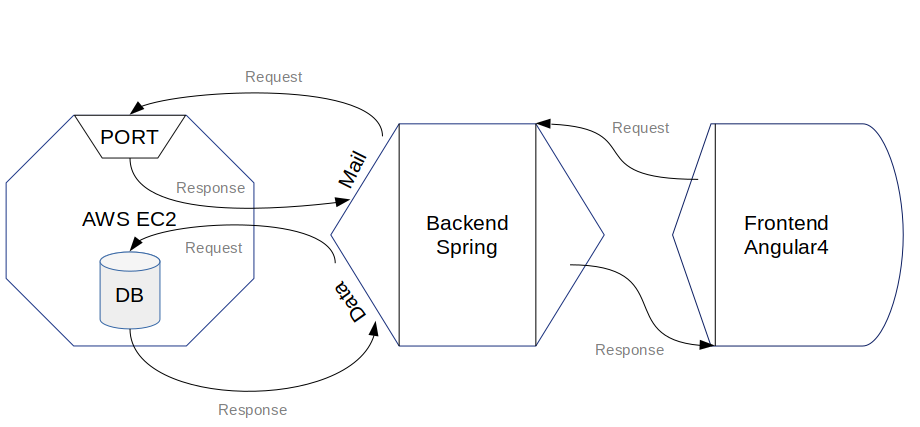
\includegraphics[scale=0.6]{basicscheme.png}}
        \caption{Взаимодействие составляющих проекта}
        \end{flushleft}
\end{figure}

Веб-приложение организованно с помощью паттерна проектирования Model-View-Control (MVC), где моделями являются разлинчные внутренние представления (напр. User, у которого есть имя, директории, логин и т.д.), control -- это сервисы и контроллеры для управления моделями (напр. у MessagesController есть метод sendMessage, который отсылает сообщение по IMAP, используя сервис MessagesService), view -- это отображение наших данных (напр. сообщений) с использованием фреймворка Angular 4.

\begin{figure}[H]
        \begin{flushleft}        \centerline{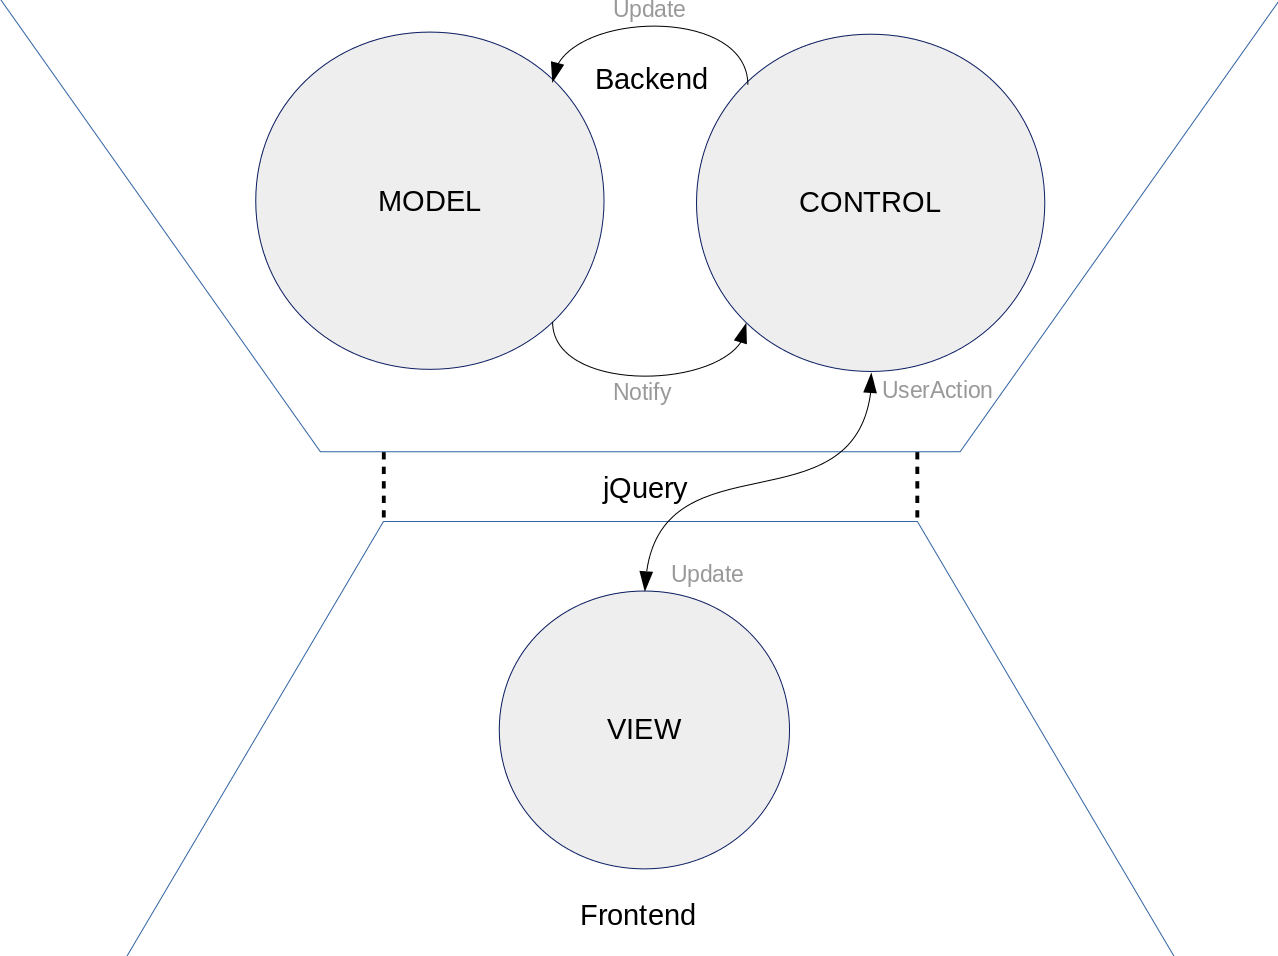
\includegraphics[scale=0.3]{mvc.png}}
        \caption{Взаимодействие составляющих проекта}
        \end{flushleft}
\end{figure}

\section{Особенности реализации}
\begin{enumerate}
\item MainController -- класс, который возвращает index.html, когда требуется mapping '/'. Нужен, чтобы выдавать экран загрузке при запуске веб-приложения.

\item UserService -- класс, который огранизует доступ в свои репозитории (данные из базы данных) и предоставляет возможность работы с ними.
	\begin{itemize}
	\item addNewUser(User user) -- добавляет нового пользователя в репозитории UserRepository
	\item getLoggedInUser() -- возвращает всю информацию, в виде класса User, о залогиненном пользователе.
	\end{itemize}
	
\item UserController -- класс, который использует класс UserService, для возвращения необходимых значений, связывая вызовы GET и POST по пути /user.
	\begin{itemize}
	\item getUserInformation() -- вызывает getLoggedInUser() класса UserService и возвращает результат в виде UserResponse, который хранит в себе информацию о пользователе в виде класса User.
	\item getLoggedInUser() -- возвращает всю информацию, ввиде класса User, о залогиненном пользователе.
	\end{itemize}
	
\item MessagesService -- класс, который хранит необходимые сведения и методы для отправки писем
	\begin{itemize}
	\item getMessages(User user) -- возвращает все доступные сообщения конкретного пользователя в качестве вектора IMAPMessage.
	\item sendMessage(String addressTo, String subject, String text, User user) -- отправляет сообщение по указанному адресу, с указанной темой, текстом от определенного пользователя.
	\end{itemize}
	
\item MessagesController -- класс, который использует класс MessagesService, для возвращения необходимых значений, связывай вызовы GET и POST по пути /messages.
	\begin{itemize}
	\item getUserInformation() -- вызывает getMessages() класса MessagesService и возвращает результат в виде MessagesResponse, который хранит в себе вектор всех сообщений.
	\item sendMessage() -- возвращает всю информацию, ввиде класса User, о залогиненном пользователе.
	\end{itemize}
	
\end{enumerate}


\end{document}